% move all configuration stuff into one file so we can focus on the content
\documentclass[aspectratio=169,hyperref={pdfpagelabels=false,colorlinks=true,linkcolor=white,urlcolor=blue},t]{beamer}

%%%%%%%%%%%%%%%%%%%%%%%%%%%%%%%%%%%%%%%%%%%%%%%%%%%%%%%%%%%%%%%%%%%%%%%%%%%%%%%%%%
%%%%%%%%%%%%%%%%%%%%%%%%%%%%%%%%%%%%%%%%%%%%%%%%%%%%%%%%%%%%%%%%%%%%%%%%%%%%%%%%%%
% packages
\usepackage{pict2e}
\usepackage{epic}
\usepackage{amsmath,amsfonts,amssymb}
\usepackage{units}
\usepackage{fancybox}
\usepackage[absolute,overlay]{textpos} 
\usepackage{media9} % avi2flv: "C:\Program Files\ffmpeg\bin\ffmpeg.exe" -i TuneFreqFilterbank.avi -b 600k -s 441x324 -r 15 -acodec copy TuneFreqFilterbank.flv
\usepackage{animate}
\usepackage{gensymb}
\usepackage{multirow}
\usepackage{silence}
\usepackage[backend=bibtex,style=ieee]{biblatex}
\AtEveryCitekey{\iffootnote{\tiny}{}}
\addbibresource{references}

%%%%%%%%%%%%%%%%%%%%%%%%%%%%%%%%%%%%%%%%%%%%%%%%%%%%%%%%%%%%%%%%%%%%%%%%%%%%%%%%%%
%%%%%%%%%%%%%%%%%%%%%%%%%%%%%%%%%%%%%%%%%%%%%%%%%%%%%%%%%%%%%%%%%%%%%%%%%%%%%%%%%%
% relative paths
\graphicspath{{graph/}}


%%%%%%%%%%%%%%%%%%%%%%%%%%%%%%%%%%%%%%%%%%%%%%%%%%%%%%%%%%%%%%%%%%%%%%%%%%%%%%%%%%
%%%%%%%%%%%%%%%%%%%%%%%%%%%%%%%%%%%%%%%%%%%%%%%%%%%%%%%%%%%%%%%%%%%%%%%%%%%%%%%%%%
% units
\setlength{\unitlength}{1mm}

%%%%%%%%%%%%%%%%%%%%%%%%%%%%%%%%%%%%%%%%%%%%%%%%%%%%%%%%%%%%%%%%%%%%%%%%%%%%%%%%%%
%%%%%%%%%%%%%%%%%%%%%%%%%%%%%%%%%%%%%%%%%%%%%%%%%%%%%%%%%%%%%%%%%%%%%%%%%%%%%%%%%%
% theme & layout
\usetheme{Frankfurt}
\beamertemplatenavigationsymbolsempty
%\setbeamertemplate{frametitle}[smoothbars theme]
\setbeamertemplate{frametitle}
{
    \begin{beamercolorbox}[ht=1.8em,wd=\paperwidth]{frametitle}
        \vspace{-.1em}%
        \hspace{.2em}{\strut\insertframetitle\strut}
        
        \hspace{.2em}\small\strut\insertframesubtitle\strut
        %\hfill
        %
\includegraphics[height=.8cm,keepaspectratio]{CenterMusicTechnology-solid-2lines-white-CoAtag}
        
    \end{beamercolorbox}
    \begin{textblock*}{100mm}(11.6cm,.7cm)
        \includegraphics[height=.8cm,keepaspectratio]{logo_GTCMT_black}
    \end{textblock*}
}

% set this to ensure bulletpoints without subsections
\usepackage{remreset}
\makeatletter
\@removefromreset{subsection}{section}
\makeatother
\setcounter{subsection}{1}

%---------------------------------------------------------------------------------
% appearance
\setbeamercolor{structure}{fg=gtgold}
\setbeamercovered{transparent} %invisible
\setbeamercolor{bibliography entry author}{fg=black}
\setbeamercolor*{bibliography entry title}{fg=black}
\setbeamercolor*{bibliography entry note}{fg=black}

%\usepackage{pgfpages}
%\setbeameroption{show notes}
%\setbeameroption{show notes on second screen=right}
%---------------------------------------------------------------------------------
% fontsize
\let\Tiny=\tiny

%%%%%%%%%%%%%%%%%%%%%%%%%%%%%%%%%%%%%%%%%%%%%%%%%%%%%%%%%%%%%%%%%%%%%%%%%%%%%%%%%%
%%%%%%%%%%%%%%%%%%%%%%%%%%%%%%%%%%%%%%%%%%%%%%%%%%%%%%%%%%%%%%%%%%%%%%%%%%%%%%%%%%
% warnings
\pdfsuppresswarningpagegroup=1
\WarningFilter{biblatex}{Patching footnotes failed}
\WarningFilter{latexfont}{Font shape}
\WarningFilter{latexfont}{Some font shapes}
\WarningFilter{gensymb}{Not defining}



\subtitle{Part 4.3: Feature Post-Processing}

%%%%%%%%%%%%%%%%%%%%%%%%%%%%%%%%%%%%%%%%%%%%%%%%%%%%%%%%%%%%%%%%%%%%%%%%%%%%
\begin{document}
    % generate title page
	

\begin{frame}
    \titlepage
    %\vspace{-5mm}
    \begin{flushright}
        \href{http://www.gtcmt.gatech.edu}{\includegraphics[height=.8cm,keepaspectratio]{logo_GTCMT_black}}
    \end{flushright}
\end{frame}


    \section[overview]{lecture overview}
        \begin{frame}{instantaneous features}{overview}
            \begin{itemize}
                \item   \textbf{text book}  
                    \begin{itemize}
                        \item   \href{http://ieeexplore.ieee.org/xpl/articleDetails.jsp?tp=&arnumber=6331120&}{\underline{\textit{Chapter 3: Instantaneous Features} (pp.~63--69)}}
                    \end{itemize}
                \item   \textbf{sources}: slides (latex) \& Matlab  
                    \begin{itemize}
                        \item   \href{https://github.com/alexanderlerch/ACA-Slides}{\underline{github repository}}
                    \end{itemize}
                \bigskip
                \item<2->   \textbf{lecture content}
                    \begin{itemize}
                        \item<2->   derived features
                        \item<3->   feature normalization
                        \item<4->   feature aggregation, transformation, and dimensionality reduction
                    \end{itemize}
            \end{itemize}
        \end{frame}

    \section[intro]{introduction}
        \begin{frame}{feature post-processing}{introduction 1/2}
            \begin{itemize}
                \item   extracting multiple instantaneous features leads to 
                    \begin{itemize}
                        \item[$\rightarrow$]   one feature vector per block, or
                        \item[$\rightarrow$]   one feature matrix per audio file
                    \end{itemize}
            \end{itemize}
            \bigskip
			\begin{eqnarray*}
				\mat{V} &=& \left[\vec{v}(0)\; 			\vec{v}(1)\; 				\ldots\;	\vec{v}(\mathcal{N}-1)\right]  \nonumber\\ 
				&=& 				 
						\left[ 
				  			\begin{array}{cccc} 
							v_0(0)					&	v_0(1) 					&	\ldots	&	v_0(\mathcal{N}-1)\\
							v_1(0)					&	v_1(1) 					&	\ldots	&	v_1(\mathcal{N}-1)\\
							\vdots					&	\vdots 					&	\ddots		&	\vdots	\\
							v_{\mathcal{F}-1}(0)	&	v_{\mathcal{F}-1}(1) 	&	\ldots	&	v_{\mathcal{F}-1}(\mathcal{N}-1)\\
							\end{array}  
						\right] 
			\end{eqnarray*}
            
            \bigskip
            \begin{footnotesize}
                dimensions:  $\mathcal{F}\times \mathcal{N}$ (number of features and number of blocks, resp.)
            \end{footnotesize}
        \end{frame}
        
        \begin{frame}{feature post-processing}{introduction 2/2}
            \question{what do we do with the feature matrix}
            
            multiple options that can be combined and depend both on the task and the classifier used
            \begin{enumerate}   
                \item   derive additional features
                \item   aggregate existing features (e.g., one feature vector per file)
                \item   reduce the number of features
                \item   ensure similar scale and distribution
            \end{enumerate}
        \end{frame}

    \section[derived]{derived features}
		\begin{frame}{feature post-processing}{examples of derived features}
            \begin{itemize}
                \item   \textbf{diff}: use the change in value
                    \begin{equation*}
                        v_{j,\Delta}(n) = v_j(n) - v_j(n-1) 
                    \end{equation*}
                \smallskip
                \item<2-> \textbf{smoothed}: remove high frequency content
                    \begin{itemize}
                        \item	 (anticausal) single-pole
                        \item	moving average
                    \end{itemize}
                \bigskip
                \item<3->   less common: non-linear combinations, e.g.
                    \begin{equation*}
                        v_{jl}(n) = v_j(n) \cdot v_l(n) 
                    \end{equation*}
            \end{itemize}
		\end{frame}

    \section[aggregation]{feature aggregation}
		\begin{frame}{feature post-processing}{feature aggregation}
            \begin{itemize}
                \item calculate \textit{summary features} from feature series: \textbf{subfeatures}
                    %\begin{itemize}
                        %\item<2->	 subfeature examples:
                            \begin{itemize}
                                \item   \textit{statistical descriptors}
                                    \begin{itemize}
                                        \item   mean, median, max, standard deviation
                                    \end{itemize}
                                        
                                \item   \textit{hand crafted }
                                    \begin{itemize}
                                        \item anything that might be meaningful --- periodicity, slope, \ldots
                                    \end{itemize}
                            %\end{itemize}
                    \end{itemize}
                \bigskip
                \item<3->   could be \textbf{hierarchical} process:
                    \begin{enumerate}
                        \item   \textit{texture window}:\\ split feature series in overlapping blocks of a few seconds length
                        \item   compute subfeatures per block
                        \item   compute subfeatures of subfeature series
                    \end{enumerate}
                \bigskip
                \item<4->   note: also compare \textit{pooling} operation in machine learning
            \end{itemize}
		\end{frame}

    \section[normalization]{feature normalization}
		\begin{frame}{feature post-processing}{normalization 1/2}
            \begin{itemize}
                \item   raw features have
                    \begin{itemize}
                        \item	different ranges and scaling factors
                        \item	possibly non-symmetric distributions
                    \end{itemize}
                \smallskip
                \item[$\Rightarrow$]<2->    potential problems with vector distances and some classifiers
                \bigskip
                \item[$\Rightarrow$]<3->    \textbf{feature normalization}
                    \begin{itemize}
                        \item \textit{standard approach} (zscore) \begin{flushright}$v_{j,\mathrm{N}}(n) = \frac{v_j(n) - \mu_{v_j}}{\sigma_{v_j}}$\end{flushright}
                        \item \textit{alternative} \begin{flushright}$  v_{j,\mathrm{N}}(n) = \frac{v_j(n) - Q_{v_j}(0.5)}{s_{v_j}}$\end{flushright}
                        with \begin{flushright}$ s_{v_j} = \sqrt{\frac{1}{\mathcal{N}}\sum\limits_{n=0}^{\mathcal{N}-1}{\big(v_j(n)-Q_{v_j}(0.5)\big)^2}}$\end{flushright}
                     \end{itemize}
            \end{itemize}
			
		\end{frame}
		\begin{frame}{feature post-processing}{normalization 2/2}
			\begin{itemize}
                \item    \textbf{alternative normalizations}
                    \begin{itemize}
                        \item   normalize range to $[0\ldots 1]$
                    \end{itemize}
				\bigskip
                \item<2->	\textbf{symmetrize pdf shape} 
                    \begin{itemize}
                        \item Box-Cox transform
                            \begin{eqnarray*}
                                v^{(\lambda)} = \left\{ 
                                                \begin{array}{ll} 
                                                    \frac{v^\lambda - 1}{\lambda}, 		& \lambda \neq 0\\ 
                                                    \vphantom{\frac{1}{1}} 	\log(v), 	& \lambda = 0 \\ 
                                                \end{array} 
                                                \right. 
                            \end{eqnarray*}
                        \item   numerical methods \ldots
                    \end{itemize}
            \end{itemize}
             
		\end{frame}
        
    \section[reduction]{feature dimensionality reduction}
		\begin{frame}{feature post-processing}{dimensionality reduction --- introduction}
            \begin{itemize}
                \item   \textbf{problem}
                    \begin{itemize}
                        \item   many ML cannot cope properly with large amounts of irrelevant features
                        \item   ML algorithms might degrade in performance
                    \end{itemize}
                \bigskip
                \item<2->   \textbf{advantages}
                    \begin{itemize}
                        \item   reducing storage requirements
                        \item   reducing training complexity
                        \item   defying the curse of dimensionality
                    \end{itemize}
                \bigskip
                \item<3->   \textbf{disadvantages}
                    \begin{itemize}
                        \item   additional workload for reduction
                        \item   adding an additional layer of model complexity
                    \end{itemize}
            \end{itemize}
		\end{frame}
		\begin{frame}{feature post-processing}{dimensionality reduction --- dimensionality issues introduction}
            problems of high-dimensional data:
            \begin{itemize}
                \item   increase in run-time
                \item   overfitting
                \item   curse of dimensionality
                \item   number of required samples (training set size)
            \end{itemize}
            \pause
			$\Rightarrow$ increasing number of input features may \textit{decrease} classification performance
			
			\begin{figure}
				\centering
				\hspace{-5mm}\vspace{-5mm}
				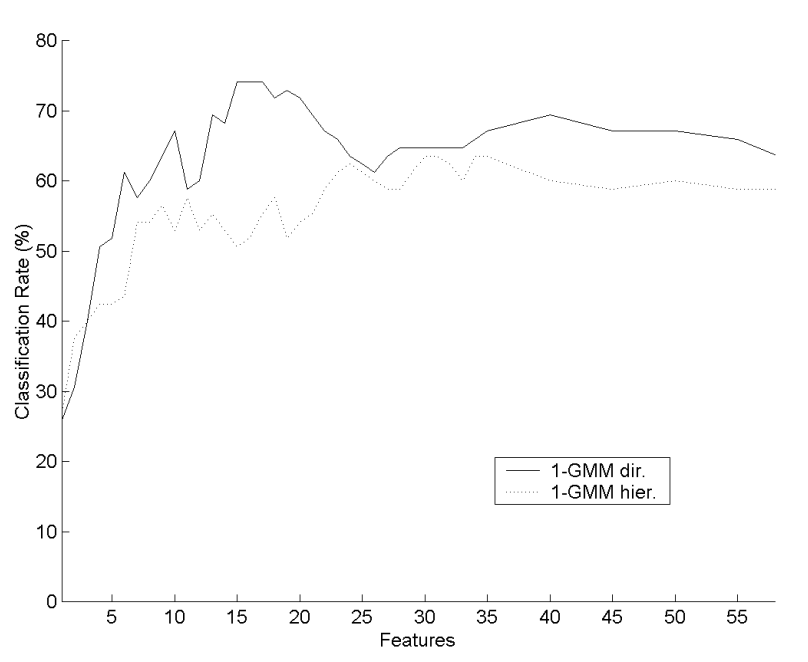
\includegraphics[scale=.2]{graph/curseofdimensionality}
			\end{figure}
		\end{frame}
		\begin{frame}{feature post-processing}{dimensionality reduction --- dimensionality issues 2/3}
            \begin{itemize}
                \item   \textbf{overfitting}:
                    \begin{itemize}
                        \item   lack of training data
                        \item   overly complex model
                        \item[$\Rightarrow$]<2-> model cannot be estimated properly
                    \end{itemize}
                    
                    \only<1-2>{
                    \figwithref{Overfitting}{\href{https://en.wikipedia.org/wiki/Overfitting}{https://en.wikipedia.org/wiki/Overfitting}}
                    %\begin{figure}
                        %\centering
                        %\includegraphics[scale=.3]{graph/overfitting}
                    %\end{figure}
                    }
                    \bigskip
                    \begin{itemize}
                        \item<3-> required training set size depends on 
                            \begin{itemize}
                                \item   classifier and its parametrization
                                \item   number of classes
                                \item   \ldots
                            \end{itemize}
                    \end{itemize}
                    \pause
                    \toremember{\textit{rule of thumb}:\\ don't bother with training sets smaller than $\mathcal{F}^2$}
			\end{itemize}
		\end{frame}
		\begin{frame}{feature post-processing}{dimensionality reduction --- dimensionality issues 3/3}
            \begin{itemize}
                \item \textbf{curse of dimensionality}: 
                    \begin{itemize}
                        \item   increasing dimensionality leads to sparse training data
                        \item   neighborhoods of data points become less concentrated
                        \item   model tends to be harder to estimate in higher-dimensional space
                        \item   applies to distance-based algorithms
                    \end{itemize}
                \item   example
                    \begin{itemize}
                        \item   uniformly distributed data 
                        \item   identify region required for \textbf{1\% of data}
                            \begin{itemize}
                                \item   2-D: 10\% of x-axis/y-axis
                                \item   3-D: 21.5\% of x-axis/y-axis/z-axis
                                \item   10-D: 63\%
                                \item   100-D: 95\%
                            \end{itemize}
                    \end{itemize}
                %\pause
                %\item   \textbf{training set density}: 
                    %example: 1NN ($9$ training samples)
                    %\only<3>{
                        %$\mathcal{F} = 1$
                    %\begin{figure}
                        %\centering
                        %\includegraphics[scale=.3]{graph/1nn-1}
                    %\end{figure}
                    %}
                    %\only<4>{
                        %$\mathcal{F} = 2$
                     %\begin{figure}
                        %\centering
                        %\includegraphics[scale=.25]{graph/1nn-2}
                    %\end{figure}
                   %}
                    %\only<5>{
                        %$\mathcal{F} = 3$
                     %\begin{figure}
                        %\centering
                        %\includegraphics[scale=.25]{graph/1nn-3}
                    %\end{figure}
                   %}
                     %\vspace{50mm}
            \end{itemize}
		\end{frame}
		\begin{frame}{feature post-processing}{dimensionality reduction --- approaches}
			\begin{itemize}
				\item	\textbf{feature subset selection}:\\ discard least helpful features
                    \pause
                    \begin{itemize}
                        \item	high ``discriminative'' or descriptive power
                        \item	non-correlation to other features
                        \item	invariance to irrelevancies
                    \end{itemize}
				\bigskip
				\item<2->	\textbf{feature space transformation}:\\ map feature space
			\end{itemize}
		\end{frame}
		\begin{frame}{feature post-processing}{manual feature selection}
            \begin{columns}[T]
            \column{.2\linewidth}
                example scatter plots of pairs of features in a multi-class scenario
            \column{.8\linewidth}
%                \begin{figure}
%                    \centering
%                    \hspace{-5mm}\vspace{-5mm}
                    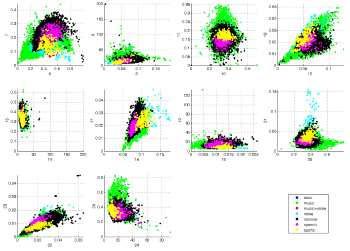
\includegraphics{noise_subfeatures}
%                \end{figure}
            \end{columns}
		\end{frame}
        
		\begin{frame}{feature post-processing}{feature subset selection: introduction}
			\begin{enumerate}
				\item	\textbf{wrapper methods}:
                    \begin{itemize}
                        \item \textit{description}
                            \begin{itemize}
                                \item  use the ``classifier'' itself to evaluate feature performance
                            \end{itemize}
                         \item<2-> \textit{advantages}
                            \begin{itemize}
                                \item   taking into account feature dependencies
                                \item   model dependency
                            \end{itemize}
                         \item<3-> \textit{disadvantages}
                            \begin{itemize}
                                \item   complexity
                                \item   risk of overfitting
                            \end{itemize}
                  \end{itemize}
				
				\bigskip
                \item<4->	\textbf{filter methods}:
                    \begin{itemize}
                        \item \textit{description}
                            \begin{itemize}
                                \item  use an objective function
                            \end{itemize}
                         \item<5-> \textit{advantages}
                            \begin{itemize}
                                \item   easily scalable
                                \item   independent of classification algorithm
                            \end{itemize}
                         \item<6-> \textit{disadvantages}
                            \begin{itemize}
                                \item   no interaction with classifier
                                \item   no feature dependencies
                            \end{itemize}
                    \end{itemize}
			\end{enumerate}
		\end{frame}

        \begin{frame}{excursion}{simple classifier~---~nearest neighbor}
            \vspace{-3mm}
            \begin{itemize}
                \item	    \textbf{training}:
                    \begin{itemize}
                        \item store feature vector (\& class label) of each training sample
                    \end{itemize}
                \item<2->	\textbf{classification}:
                    \begin{itemize}
                        \item for new file/feature vector, detect \textit{closest training point}
                        \item   choose closest point's class as result
                    \end{itemize}
            \end{itemize}
            \vspace{-4mm}
            \only<1>{
                \figwithmatlab{Scatter}
            }
            \only<2->{
                \figwithref{Scatter-nn}{matlab source: matlab/displayScatter.m}
            }
        \end{frame}
        
		\begin{frame}{feature post-processing}{feature subset selection: wrapper methods 1/2}
			\begin{enumerate}
				\item	\textbf{single variable classification}:
                    \begin{itemize}
                        \item   \textit{procedure}
                            \begin{itemize}
                                \item   evaluate each feature individually
                                \item   choose the top $N$
                            \end{itemize}
                        \item<2->  \textit{complexity} 
                            \begin{itemize}
                                \item   subsets to test: $\mathcal{F}$
                            \end{itemize}
                        \item<3->   \textit{challenges}
                            \begin{itemize}
                                \item	inter-feature correlation is not considered
                                \item	feature combinations are not considered
                            \end{itemize}
                    \end{itemize}
				\bigskip 
                \item<4->	\textbf{brute force subset selection}
                    \begin{itemize}
                        \item   \textit{procedure}
                            \begin{itemize}
                                \item   evaluate all possible feature combinations
                                \item   choose the optimal combination
                            \end{itemize}
                        \item<5->  \textit{complexity} 
                            \begin{itemize}
                                \item   subsets to test: $2^\mathcal{F}$
                            \end{itemize}
                        \item<6->   \textit{challenges}
                            \begin{itemize}
                                \item	best solution, but
                                \item	not feasible with large number of features
                            \end{itemize}
                    \end{itemize}
			\end{enumerate}
		\end{frame}
		\begin{frame}{feature post-processing}{feature subset selection: wrapper methods 2/2}
            \vspace{-2mm}
			\begin{enumerate}
                \setcounter{enumi}{3}
				\item	\textbf{sequential forward selection}
                    \begin{itemize}
                        \item   \textit{procedure}
                            \begin{enumerate}
                                \item	init: empty feature subset $\mathcal{V}_\mathrm{s} = {\emptyset}$
                                \item<2->	find feature $v_j$ maximizing objective function
                                            \begin{equation*}
                                                v_j = \argmax_{\forall j | v_j \notin \mathcal{V}_\mathrm{s}} J({\mathcal{V}_\mathrm{s}} \bigcup v_j) 
                                            \end{equation*}
                                \item<3->	add feature $v_j$ to $\mathcal{V}_\mathrm{s}$ 
                                \item<4->	go to step $2$
                            \end{enumerate}
                        \item<5->   \textit{challenges}
                            \begin{itemize}
                                \item	in theory, the optimal solution may be missed
                            \end{itemize}
                    \end{itemize}
					
				\bigskip
                \item<6->	\textbf{sequential backward elimination}
                    \begin{itemize}
                        \item   \textit{procedure}
                            \begin{enumerate}
                                \item	init: full feature set
                                \item<7->	find feature $v_j$ with the least impact on objective function
                                \item<8->	discard feature $v_j$
                                \item<9->	go to step $2$
                            \end{enumerate}
                        \item<10->   \textit{challenges}
                            \begin{itemize}
                                \item	complex with a large number of features
                            \end{itemize}
                    \end{itemize}
			\end{enumerate}
		\end{frame}
		\begin{frame}{feature post-processing}{feature space transformation: PCA introduction}
            \begin{itemize}
                \item   \textbf{objective}
                    \begin{itemize}
                        \item   map features to new coordinate system
                            \begin{equation*}\label{eq:pca_an}
                                \vec{u}(n) = \mat{T}^\mathrm{T}\cdot\vec{v}(n) 
                            \end{equation*}
                            \begin{itemize}
                                \item   $\vec{u}(n)$: transformed features (same dimension as $\vec{v}(n)$)
                                \item   $\mat{T}$: transformation matrix ($\mathcal{F}\times\mathcal{F}$)	
                                    \begin{equation*}
                                        \mat{T} =   \left[ 
                                                        \begin{array}{cccc}
                                                        \vec{c}_0 & \vec{c}_1 & \ldots & \vec{c}_{\mathcal{F}-1}\\
                                                        \end{array}  
                                                    \right] 
                                    \end{equation*}
                            \end{itemize}
                    \end{itemize}
                \item<2->   \textbf{properties}
                    \begin{itemize}
                        \item	$\vec{c}_0$ points in the direction of  highest \emph{variance}
                        \item<3->	variance concentrated in as few output components as possible
                        \item<4->	$\vec{c}_i$ orthogonal
                                \begin{equation*}
                                    \vec{c}_i^\mathrm{T}\cdot \vec{c}_j = 0\quad \forall\enspace i \neq j
                                \end{equation*}
                        \item<5->	transformation is invertible
                                \begin{equation*}\label{eq:pca_syn}
                                    \vec{v}(n) = \mat{T}\cdot\vec{u}(n)
                                \end{equation*}
                    \end{itemize}
            \end{itemize}
		\end{frame}
		\begin{frame}{feature post-processing}{feature space transformation: PCA visualization}
			\figwithmatlab{Pca}
			
			\vspace{-5mm}
			\pause
			calculation of the transformation matrix
			\begin{enumerate}
				\item	compute covariance matrix $\mat{R}$
                    \begin{equation*}
						\mat{R} = \mathcal{E}\lbrace(V-\mathcal{E}\lbrace V\rbrace)(V-\mathcal{E}\lbrace V\rbrace)\rbrace%\frac{1}{\mathcal{F}-1}\cdot \left(\vec{v} - \vec{\mu}_v\right)\left(\vec{v}^\mathrm{T} - \vec{\mu}^\mathrm{T}_v\right)
					\end{equation*}
				\item	choose eigenvectors as axes for the new coordinate system
			\end{enumerate}
		\end{frame}

		\begin{frame}{feature post-processing}{PCA example}
            \only<1>{
                \textbf{pca input}
                \figwithref{PcaExample_input}{matlab source: matlab/displayPcaExample.m}
            }
            \only<2>{
                \textbf{pca output}
                \figwithref{PcaExample_output}{matlab source: matlab/displayPcaExample.m}
            }
             \only<3>{
            \textbf{pca eigenvalues}
                \figwithref{PcaExample_latent}{matlab source: matlab/displayPcaExample.m}
            }
            \only<4>{
            \textbf{pca transformation matrix}
                    \begin{equation}\left[ 
				  			\begin{array}{cccccc} 
   -0.4187 &   0.3467  & -0.4569  &  0.4143 &  -0.1271 &  -0.5549\\
   -0.3908 &   0.1815  &  0.8136  & -0.0289 &   0.2060 &  -0.3304\\
   -0.4516 &   0.3384  &  0.0859  &  0.2413 &  -0.2919 &   0.7285\\
   -0.4337 &   0.1699  & -0.3337  & -0.7243 &   0.3747 &   0.0816\\
    0.3802 &   0.5599  & -0.0381  &  0.2808 &   0.6622 &   0.1524\\
    0.3679 &   0.6245  &  0.0956  & -0.4071 &  -0.5267 &  -0.1495\nonumber
                             \end{array}  
		        	\right]         \end{equation}   }
            \only<5>{
            \textbf{pca transformation matrix}
                    \begin{equation}\left[ 
				  			\begin{array}{cccccc} 
   \textcolor{gtgold}{-0.4187} &   0.3467  & \textcolor{gtgold}{-0.4569}  &  0.4143 &  -0.1271 &  \textcolor{gtgold}{-0.5549}\\
   -0.3908 &   0.1815  &  \textcolor{gtgold}{0.8136}  & -0.0289 &   0.2060 &  -0.3304\\
   \textcolor{gtgold}{-0.4516} &   0.3384  &  0.0859  &  0.2413 &  -0.2919 &   \textcolor{gtgold}{0.7285}\\
   \textcolor{gtgold}{-0.4337} &   0.1699  & -0.3337  & \textcolor{gtgold}{-0.7243} &   0.3747 &   0.0816\\
    0.3802 &   \textcolor{gtgold}{0.5599}  & -0.0381  &  0.2808 &   \textcolor{gtgold}{0.6622} &   0.1524\\
    0.3679 &   \textcolor{gtgold}{0.6245}  &  0.0956  & -0.4071 &  \textcolor{gtgold}{-0.5267} &  -0.1495\nonumber
                             \end{array}  
		        	\right]         \end{equation}   }
            
		\end{frame}
		\begin{frame}{feature post-processing}{feature space transformation: PCA exercise}
            \matlabexercise{compute the principle components}
                \begin{enumerate}
                    \item   extract 3 features: Spectral Centroid, Spectral Flux, and RMS
                    \item   normalize the features
                    \item   compute the principle components (\texttt{pca()} statistics toolbox)
                    \item   analyze the transformation matrix and the variances --- what can you learn about the input features
                \end{enumerate}
		\end{frame}

    \section[summary]{lecture summary}
        \begin{frame}{summary}{lecture content}
            \begin{enumerate}
                \item   name examples for typical ways of computing derived features      
                \smallskip
                \item<2->   why is more features not always better
                \smallskip
                \item<3->   what is the difference between feature selection and feature mapping
                \smallskip
                \item<4->   describe two ways of selecting features
                \smallskip
                \item<5->   what is PCA and what are the advantages
            \end{enumerate}
        \end{frame}
\end{document}

